\chapter{Research}\label{research}
In this chapter or in these chapters you write/ show all the details that are required to \textquote {prove} your hypothesis. This should be sufficiently detailed and precise such that your fellow students are able to repeat the research and establish the same results and conclusions. 

When using large images or models you can use the appendix to improve the readability of your thesis: See the appendix \ref{appendix}. 

When you want to use a large image you might want to rotate the image, you can use boxes to use the same image in several ways:

%First create a box for the image
\newsavebox{\BoxName}
\sbox{\BoxName}{%
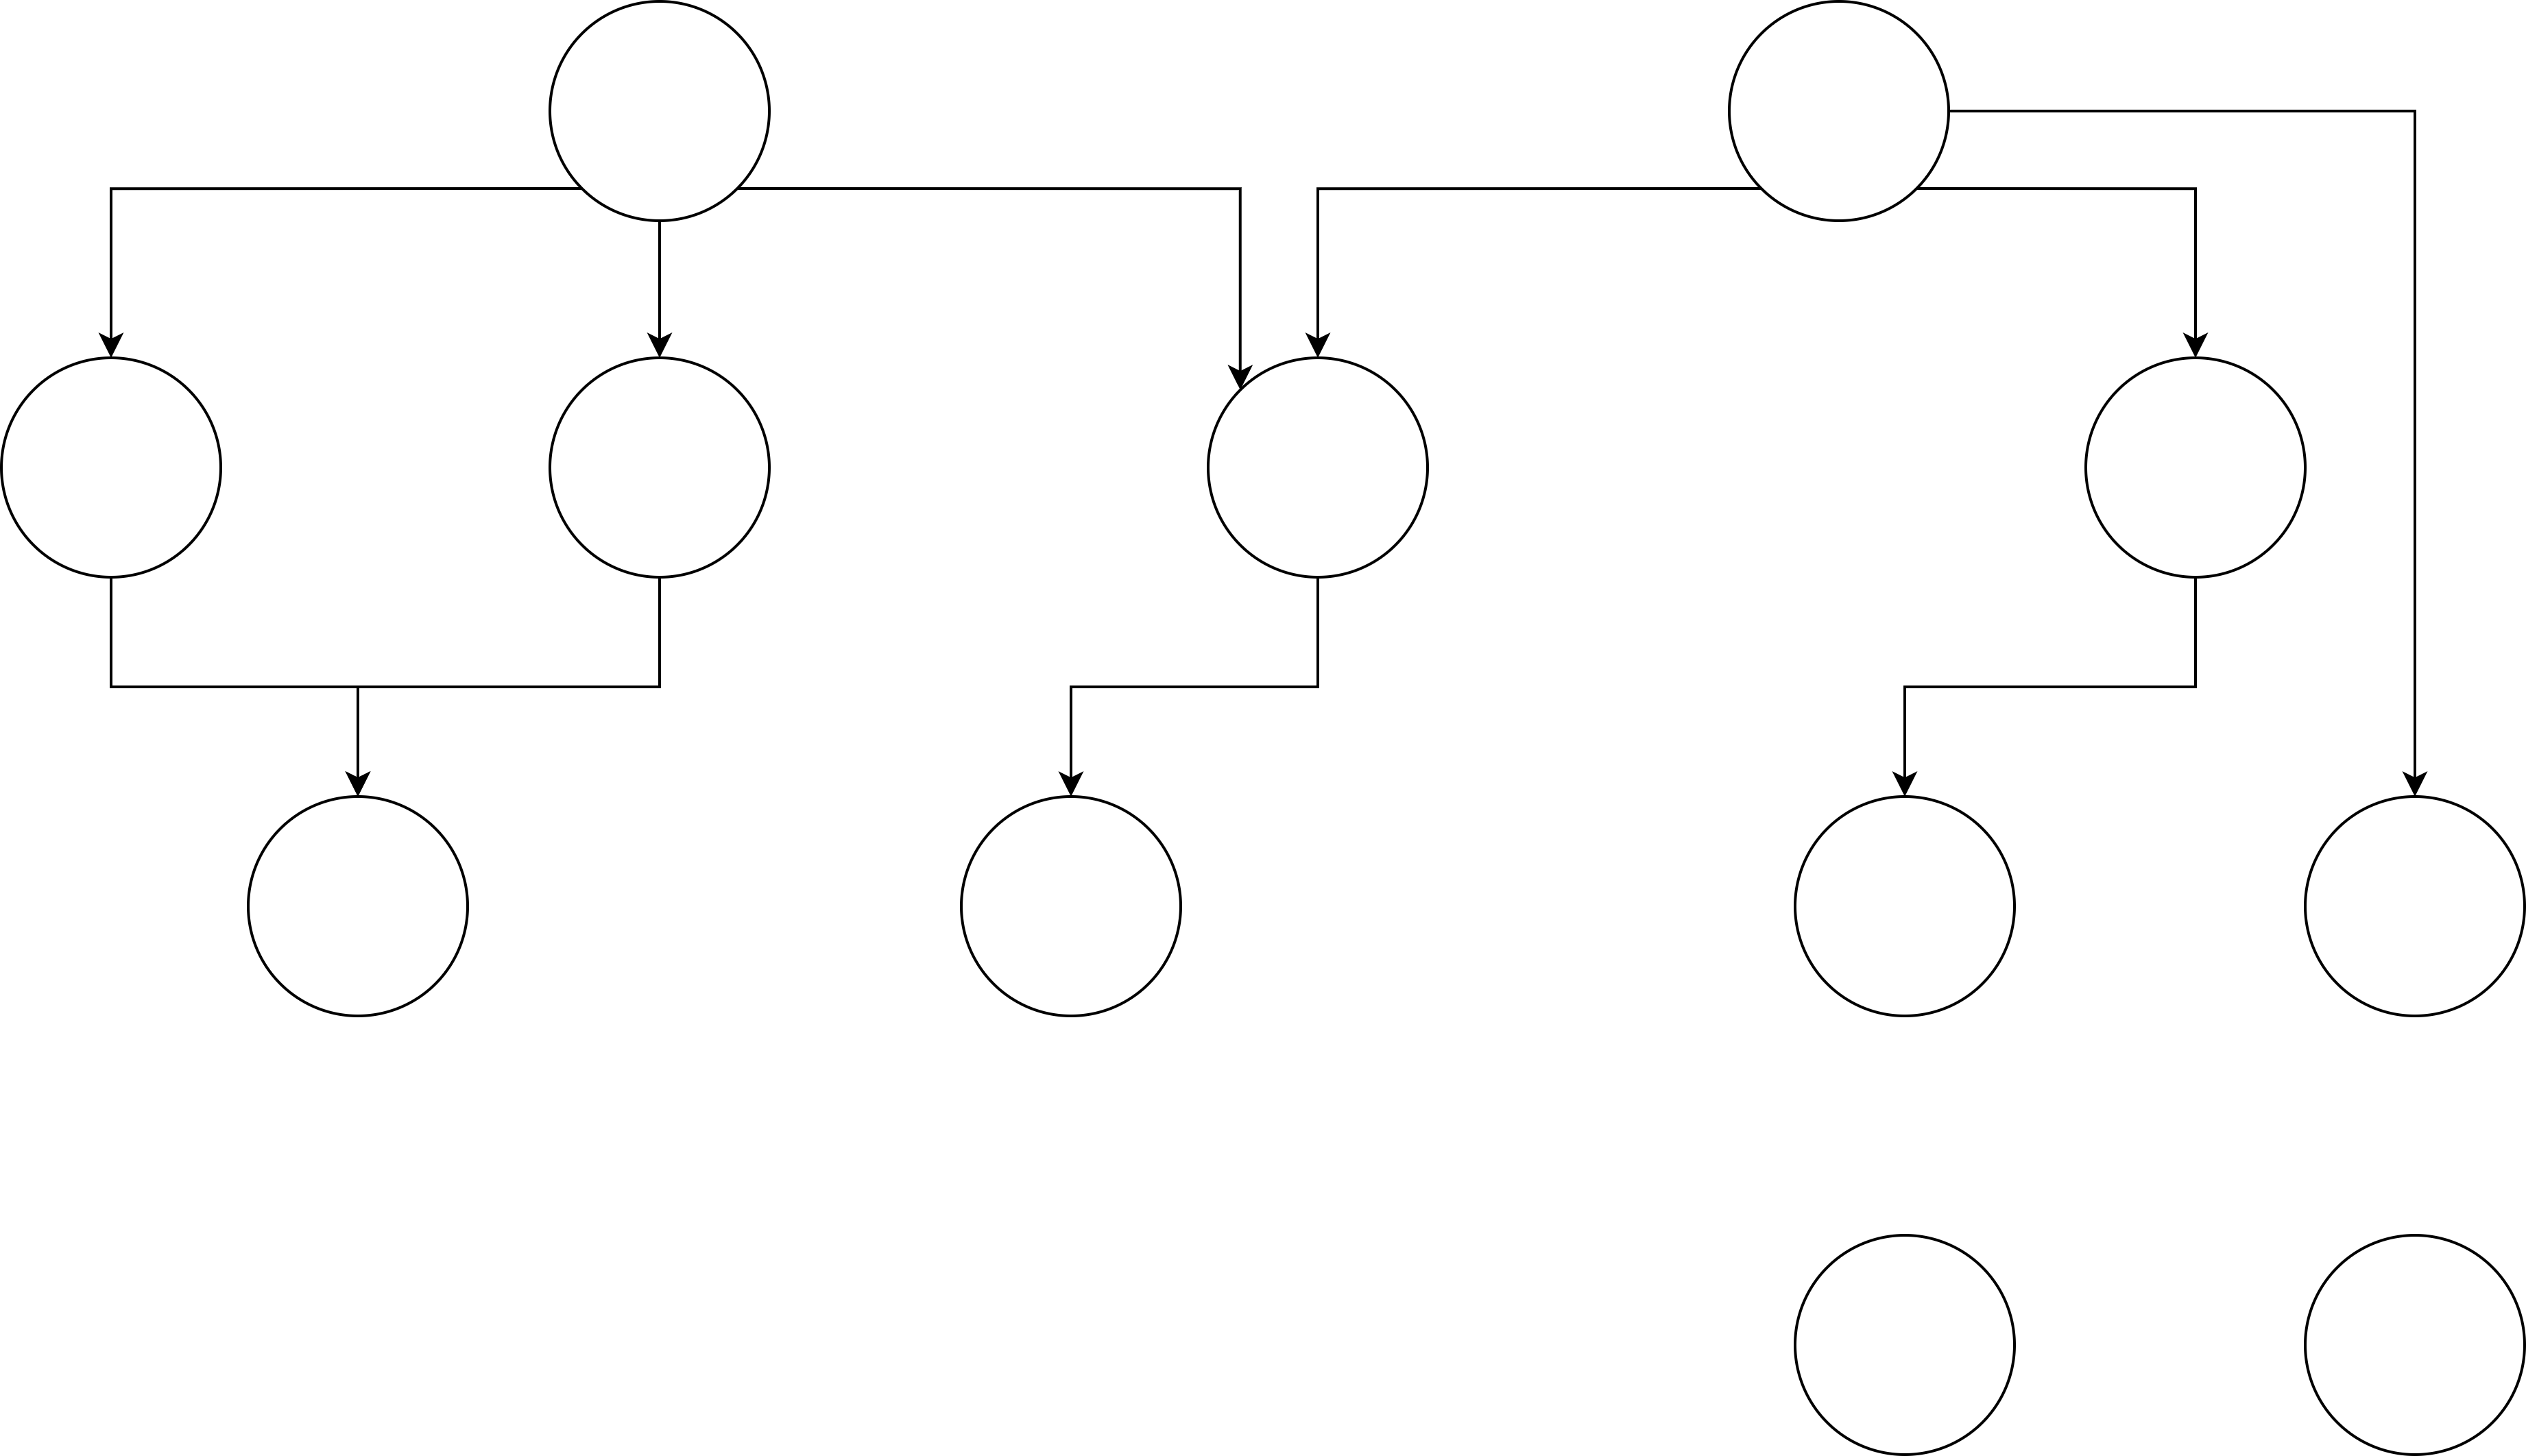
\includegraphics{Imgs/Example_model.png}
}

%The in normal text
\begin{figure}[H]
    \centerline{\resizebox{\textwidth}{!}{\usebox{\BoxName}}}
    \caption{An example image}
    \label{fig:example_image}
\end{figure}

% The rotated image (Usually put in the appendix)
\begin{sidewaysfigure}
\centerline{\resizebox{!}{0.7\textheight}{\usebox{\BoxName}}}
\caption{Rotated example image}
\label{fig:rotated_image}
\end{sidewaysfigure}